\section{Moment Realizability for the Fermionic Two-Moment Model}
\label{sec:realizability}

Our goal is to simulate massless fermions (e.g., neutrinos) and study their interactions with matter.  
The principal objective is to obtain the fermionic distribution function $f$ (or moments of $f$ as in the two-moment model employed here).  
The Pauli exclusion principle requires the distribution function to satisfy the condition $0 \le f \le 1$, which puts restrictions on the admissible values for the moments of $f$.  
In this paper, we seek to design a numerical method for solving the system of moment equations given by Eq.~\eqref{eq:momentEquations} that preserves realizability of the moments; i.e., the moments evolve within the set of admissible values as dictated by Pauli's exclusion principle.  
(Since we are only concerned with the angular dependence of $f$ in this section, we simplify the notation by suppressing the $\vect{z}$ and $t$ dependence and write $f(\omega,\vect{z},t)=f(\omega)$.)  

\modified{
We let
\begin{equation}
  \mathfrak{R} := \left\{\,f~|~0\le f \le 1 ~\text{and}~0<\f{1}{4\pi}\int_{\bbS^{2}}f\,d\omega<1\,\right\},
\end{equation}
and begin with the following definition of moment realizability.}  
\begin{define}
  \modified{The moments $\vect{\cM}=\big(\cJ,\vect{\cH}\big)^{T}$ are realizable if they can be obtained from a distribution function $f(\omega)\in\mathfrak{R}$.}  
  %satisfying $0 < f(\omega) < 1~\forall~\omega\in\bbS^{2}$.  
  The set of all realizable moments $\cR$ is
  \begin{equation}
    \cR:=\big\{\,\vect{\cM}=\big(\cJ,\vect{\cH}\big)^{T}~|~\cJ\in(0,1)~\text{and}~\gamma(\vect{\cM}) > 0\,\big\},
    \label{eq:realizableSet}
  \end{equation}
  where we have defined the concave function $\gamma(\vect{\cM})\equiv(1-\cJ)\cJ-|\vect{\cH}|$.  
  \label{def:momentRealizability}
\end{define}
\begin{rem}
  Following \cite{lareckiBanach_2011}, in Definition~\ref{def:momentRealizability}, and in the rest of this paper, we exclude the cases $f=0$ and $f=1$ almost everywhere (a.e.) on $\bbS^{2}$, which would give $\cJ=0$, $\vect{\cH}=0$ and $\cJ=1$, $\vect{\cH}=0$, respectively.  
\end{rem}
\modified{
\begin{rem}
  The conditions in Eq.~\eqref{eq:realizableSet} are necessary and sufficient for the moments to be realizable \cite[Theorem 7.1]{banachLarecki_2017a}.  (See also \cite{lareckiBanach_2011,banachLarecki_2013}.)
\end{rem}
}

%The algebraic constraints in Eq.~\eqref{eq:realizableSet} are proven in \cite{banachLarecki_2017a}.  
%\begin{lemma}
%  Suppose that $0 < f(\omega) < 1~\forall~\omega\in\bbS^{2}$.  
%  Then the moments $\vect{\cM}=(\cJ,\vect{\cH})^{T}$, defined as in Eq.~\eqref{eq:angularMoments}, satisfy $0 < \cJ < 1$ and $\big(1-\cJ\big)\,\cJ-|\vect{\cH}| > 0$. 
%  \label{lem:MomentRealizable} 
%\end{lemma}

%\begin{define}
%  For the fermion two-moment model, the realizable set is
%  \begin{equation}
%    \cR:=\big\{\,\vect{\cM}=\big(\cJ,\vect{\cH}\big)^{T}~|~\cJ\in(0,1)~\text{and}~\gamma(\vect{\cM})\equiv(1-\cJ)\cJ-|\vect{\cH}| > 0\,\big\}.
%    \label{eq:realizableSet}
%  \end{equation}
%\end{define}

\begin{lemma}
  The realizable set $\cR$ is convex.  
\end{lemma}
\begin{proof}
%  In order to prove that $\cR$ is convex, it is sufficient to show that any convex combination of elements in $\cR$ also belongs to $\cR$.  
  Let $\vect{\cM}_{a}=\big(\cJ_{a},\vect{\cH}_{a}\big)^{T}$ and $\vect{\cM}_{b}=\big(\cJ_{b},\vect{\cH}_{b}\big)^{T}$ be two arbitrary elements in $\cR$, and let $\vect{\cM}_{c} = \theta\,\vect{\cM}_{a} + (1-\theta)\,\vect{\cM}_{b}$, with $0\leq\theta\leq1$.
  The first component of $\vect{\cM}_{c}$ is
  \begin{equation*}
    \cJ_{c} = \theta\,\cJ_{a} + (1-\theta)\,\cJ_{b}.
  \end{equation*}
  Since $\cJ_{a},\cJ_{b} \in (0,1)$, it follows that $\cJ_{c} \in (0,1)$.  
  Concavity of $\gamma$ implies that
%  Since $\cJ_{a},\cJ_{b} \in (0,1)$, it is straightforward to verify that
  \begin{equation*}
  \gamma(\vect{\cM}_{c}) \geq \theta\,\gamma(\vect{\cM}_{a}) + (1-\theta)\,\gamma(\vect{\cM}_{b}) > 0.
  \end{equation*}
  Hence, $\vect{\cM}_{c}\in\cR$.
\end{proof}

Figure~\ref{fig:RealizableSetFermionic} illustrates the geometry of the convex set $\cR$ in the $(\cH,\cJ)$-plane (light blue region).  
The boundary $\partial\cR$ (black curves) is given by $\gamma(\vect{\cM})=0$.  
The realizable domain of positive distribution functions, $\cR^{+}$ (no upper bound on $f$), which is a convex cone defined by
\begin{equation}
  \cR^{+}:=\big\{\,\vect{\cM}=\big(\cJ,\vect{\cH}\big)^{T}~|~\cJ > 0~\text{and}~\cJ > |\vect{\cH}|\,\big\}, 
  \label{eq:realizableSetPositive}
\end{equation}
is partially shown as the light red region above the red lines, which mark the boundary of $\cR^{+}$ (denoted $\partial\cR^{+}$).  
The realizable set $\cR$ is a bounded subset of $\cR^{+}$.  
%The realizable domains $\cR$ and $\cR^{+}$ overlap for low particle densities ($\cJ\ll1$), but for larger values of $\cJ$, the realizable domain of particles governed by Fermi-Dirac statistics is much more restricted than that of particles described by positive distribution functions with no upper bound.  

\begin{figure}[H]
  \centering
  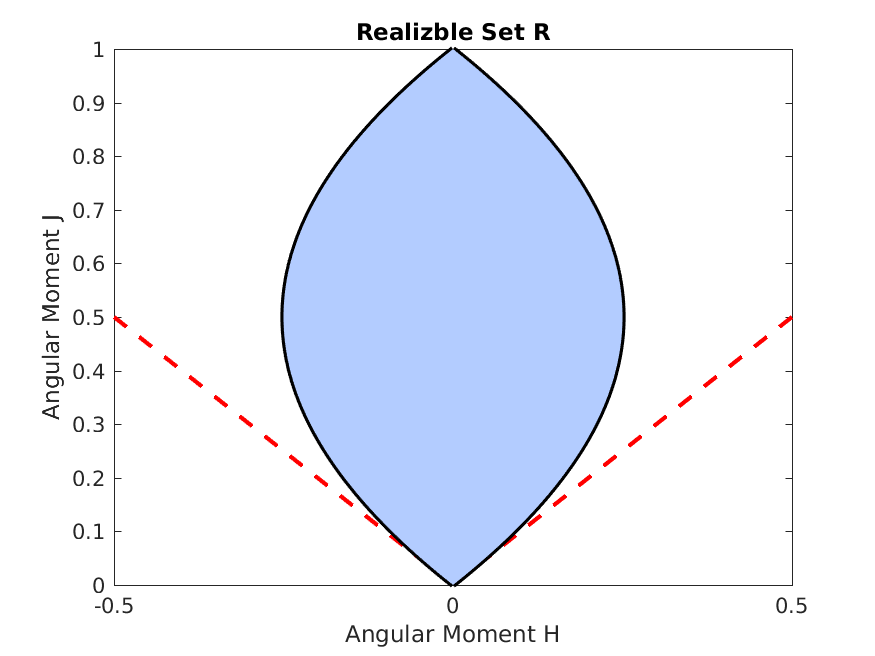
\includegraphics[width=1.0\linewidth]{figures/RealizableSetFermionic}
  \caption{Illustration of the realizable set $\cR$ (light blue region) defined in Eq.~\eqref{eq:realizableSet}.  
  The black lines define the boundary $\partial\cR$, while the red lines indicate the boundary of the realizable set $\cR^{+}$ (light red region) defined in Eq.~\eqref{eq:realizableSetPositive}.}
  \label{fig:RealizableSetFermionic}
\end{figure}

For the realizability-preserving scheme developed in Section~\ref{sec:realizableDGIMEX}, we state some additional results.  
Lemma~\ref{lem:explicitStep} is used to help prove the realizability-preserving property of explicit steps in the IMEX scheme, while Lemmas~\ref{lem:implicitStep} and \ref{lem:correctionStep} are used to prove realizability-preserving properties of implicit steps.  
\begin{lemma}
  Let $\big\{\cJ_{a},\vect{\cH}_{a},\vect{\cK}_{a}\big\}$ and $\big\{\cJ_{b},\vect{\cH}_{b},\vect{\cK}_{b}\big\}$ be moments defined as in Eq.~\eqref{eq:angularMoments} with distribution functions $f_{a}$ and $f_{b}$, respectively, such that $f_{a}(\omega),f_{b}(\omega)\in(0,1)\,\forall\,\omega\in\bbS^{2}$.  
  Let $\Phi^{\pm}(\vect{\cM},\vect{\cK})=\f{1}{2}\big(\vect{\cM}\pm\widehat{\vect{e}}\cdot\vect{\cF}\big)$, where $\widehat{\vect{e}}\in\bbR^{3}$ is an arbitrary unit vector, and $\widehat{\vect{e}}\cdot\vect{\cF}=\big(\widehat{\vect{e}}\cdot\vect{\cH},\widehat{\vect{e}}\cdot\vect{\cK}\big)^{T}$.  
  Then
  \begin{equation*}
    \vect{\cM}_{ab} \equiv \Phi^{+}(\vect{\cM}_{a},\vect{\cK}_{a})+\Phi^{-}(\vect{\cM}_{b},\vect{\cK}_{b})\in\cR.
  \end{equation*}
  \label{lem:explicitStep}
\end{lemma}
\begin{proof}
  The components of $\vect{\cM}_{ab}$ are
  \begin{equation*}
    \cJ_{ab}=\f{1}{4\pi}\int_{\bbS^{2}}f_{ab}(\omega)\,d\omega
    \quad\text{and}\quad
    \vect{\cH}_{ab}=\f{1}{4\pi}\int_{\bbS^{2}}f_{ab}(\omega)\,\vect{\ell}(\omega)\,d\omega,
  \end{equation*}
  where $f_{ab}(\omega)=\vartheta\,f_{a}(\omega)+(1-\vartheta)\,f_{b}(\omega)$ and $\vartheta(\omega)=(1+\widehat{\vect{e}}\cdot\vect{\ell}(\omega))/2\in[0,1]$.  
  Then, since $f_{ab}(\omega)\in(0,1)\,\forall\,\omega\in\bbS^{2}$, it follows that $\vect{\cM}_{ab}\in\cR$.  
\end{proof}

\begin{lemma}
  Let $\vect{\cM}_{a}=(\cJ_{a},\vect{\cH}_{a})^{T}\in\cR$ and $\alpha>0$.  
  Let $\vect{\cM}_{b}=(\cJ_{b},\vect{\cH}_{b})^{T}$ satisfy
  \begin{equation}
    \vect{\cM}_{b}=\vect{\cM}_{a}+\alpha\,\vect{\cC}(\vect{\cM}_{b}), 
    \label{eq:implicitStep}
  \end{equation}
  where $\vect{\cC}(\vect{\cM})=\vect{\eta}-\vect{\cD}\,\vect{\cM}$ is the collision term in Eq.~\eqref{eq:collisionTermMoments}.  
  Then $\vect{\cM}_{b}\in\cR$.  
  \label{lem:implicitStep}
\end{lemma}
\begin{proof}
  Solving Eq.~\eqref{eq:implicitStep} for $\vect{\cM}_{b}$ gives $\vect{\cM}_{b} = \big(\vect{I}+\alpha\,\vect{\cD}\big)^{-1}\big(\vect{\cM}_{a}+\alpha\,\vect{\eta}\big)$.  
  The first component of $\vect{\cM}_{b}$ can be written as
  \begin{equation*}
    \cJ_{b}=\f{1}{4\pi}\int_{\bbS}f_{b}(\omega)\,d\omega,
  \end{equation*}
  where $f_{b}(\omega)=\zeta\,f_{a}(\omega)+(1-\zeta)\,f_{0}$, $\zeta=1/(1+\alpha\,\xi)\in[0,1]$, and $f_{0}$ and $\xi$ are defined in Eq.~\eqref{eq:collisionTerm} in Section~\ref{sec:model}.  
  Then, since $f_{b}(\omega)\in(0,1)\,\forall\,\omega\in\bbS^{2}$, $\cJ_{b}\in(0,1)$.  
  Meanwhile, 
  \begin{equation*}
    \vect{\cH}_{b}=\f{(1+\alpha\,\xi)}{(1+\alpha)}\,\widetilde{\vect{\cH}}_{b},
    \quad\text{where}\quad
    \widetilde{\vect{\cH}}_{b}=\f{1}{4\pi}\int_{\bbS^{2}}f_{b}(\omega)\,\vect{\ell}(\omega)\,d\omega.  
  \end{equation*}
  It follows that $\widetilde{\vect{\bcM}}_{b}=(\cJ_{b},\widetilde{\vect{\cH}}_{b})^{T}\in\cR$.  
  Then, since $0\le\xi\le1$, $|\vect{\cH}_{b}|\le|\widetilde{\vect{\cH}}_{b}| < (1-\cJ_{b})\,\cJ_{b}$.  
\end{proof}

\begin{lemma}
  Let $\vect{\cM}_{a}=(\cJ_{a},\vect{\cH}_{a})^{T}\in\cR$ and $\alpha>0$.  
  Let $\vect{\cM}_{b}$ satisfy
  \begin{equation*}
    \vect{\cM}_{b}=\vect{\cM}_{a}+\alpha\,\vect{\cD}\,\vect{\cC}(\vect{\cM}_{b}),    
  \end{equation*}
  where $\vect{\cD}$ and $\vect{\cC}(\vect{\cM})$ are given by Eq.~\eqref{eq:collisionTermMoments}.  
  Then $\vect{\cM}_{b}\in\cR$.  
  \label{lem:correctionStep}
\end{lemma}
The proof of Lemma~\ref{lem:correctionStep} follows along the same lines as the proof of Lemma~\ref{lem:implicitStep} and is omitted.  
